%% ============================================================
%% SAMBP Digital Twin Protection Lab
%% Research Gap Analysis & TR Roadmap — Internal Working Document
%% Author : Anoop V Eluvathingal, IIT Madras
%% Date   : April 2026
%% Usage  : pdflatex sambp_roadmap.tex  (standalone, no class deps)
%% ============================================================
\documentclass[11pt, a4paper]{article}

%% ── Packages ────────────────────────────────────────────────
\usepackage[a4paper, top=25mm, bottom=28mm, left=22mm, right=22mm]{geometry}
\usepackage{amsmath, amssymb}
\usepackage{booktabs}
\usepackage{longtable}
\usepackage{array}
\usepackage{multirow}
\usepackage{xcolor}
\usepackage{colortbl}
\usepackage{tabularx}
\usepackage{enumitem}
\usepackage{titlesec}
\usepackage{fancyhdr}
\usepackage{parskip}
\usepackage{microtype}
\usepackage{hyperref}
\usepackage{fontenc}
\usepackage{inputenc}
\usepackage{lmodern}
\usepackage{mdframed}
\usepackage{tikz}
\usetikzlibrary{positioning, arrows.meta, shapes.geometric, calc}

%% ── Colours ─────────────────────────────────────────────────
\definecolor{navy}{HTML}{0b1e3d}
\definecolor{blue}{HTML}{1a6fdf}
\definecolor{cyan}{HTML}{0891b2}
\definecolor{amber}{HTML}{d97706}
\definecolor{green}{HTML}{16a34a}
\definecolor{red}{HTML}{dc2626}
\definecolor{slate}{HTML}{64748b}
\definecolor{lightgray}{HTML}{f1f5f9}
\definecolor{rowalt}{HTML}{f8fafc}
\definecolor{tier1bg}{HTML}{fef2f2}
\definecolor{tier2bg}{HTML}{fffbeb}
\definecolor{tier3bg}{HTML}{f0f9ff}
\definecolor{headerbg}{HTML}{1e3a5f}

%% ── Section formatting ──────────────────────────────────────
\titleformat{\section}
  {\large\bfseries\color{navy}}
  {\thesection.}{0.6em}{}[\vspace{-4pt}\textcolor{blue}{\rule{\linewidth}{1.5pt}}]

\titleformat{\subsection}
  {\normalsize\bfseries\color{navy}}
  {\thesubsection.}{0.5em}{}

\setlist[itemize]{leftmargin=1.4em, itemsep=2pt, topsep=4pt}
\setlist[enumerate]{leftmargin=1.4em, itemsep=2pt, topsep=4pt}

%% ── Header / footer ─────────────────────────────────────────
\pagestyle{fancy}
\fancyhf{}
\fancyhead[L]{\small\textcolor{slate}{SAMBP Digital Twin Lab — Internal Roadmap}}
\fancyhead[R]{\small\textcolor{slate}{Confidential Draft · April 2026}}
\fancyfoot[C]{\small\textcolor{slate}{\thepage}}
\renewcommand{\headrulewidth}{0.3pt}
\renewcommand{\headrule}{\textcolor{blue}{\hrule height 0.3pt}}

%% ── Hyperref ────────────────────────────────────────────────
\hypersetup{
  colorlinks=true,
  linkcolor=blue,
  urlcolor=cyan,
  pdftitle={SAMBP Research Gap Analysis and TR Roadmap},
  pdfauthor={Anoop V Eluvathingal},
}

%% ── Column types ─────────────────────────────────────────────
\newcolumntype{L}[1]{>{\raggedright\arraybackslash}p{#1}}
\newcolumntype{C}[1]{>{\centering\arraybackslash}p{#1}}

%% ── Macros ───────────────────────────────────────────────────
\newcommand{\tier}[1]{%
  \ifnum#1=1
    \colorbox{red!15}{\textcolor{red}{\textbf{\footnotesize T1}}}%
  \else\ifnum#1=2
    \colorbox{amber!20}{\textcolor{amber}{\textbf{\footnotesize T2}}}%
  \else
    \colorbox{cyan!12}{\textcolor{cyan}{\textbf{\footnotesize T3}}}%
  \fi\fi
}
\newcommand{\effortcell}[1]{\textcolor{slate}{\footnotesize #1}}
\newcommand{\depcell}[1]{\textcolor{slate}{\footnotesize\textit{#1}}}
\newcommand{\trnum}[1]{\textbf{TR-#1}}
\newcommand{\status}[1]{%
  \ifnum#1=1
    \colorbox{green!15}{\textcolor{green}{\textbf{\footnotesize Done}}}%
  \else\ifnum#1=2
    \colorbox{blue!12}{\textcolor{blue}{\textbf{\footnotesize Active}}}%
  \else
    \colorbox{slate!12}{\textcolor{slate}{\textbf{\footnotesize Planned}}}%
  \fi\fi
}

%% ── Infobox ──────────────────────────────────────────────────
\newmdenv[
  linecolor=blue,
  linewidth=1.2pt,
  leftline=true, topline=false, rightline=false, bottomline=false,
  backgroundcolor=blue!4,
  innerleftmargin=10pt,
  innerrightmargin=8pt,
  innertopmargin=6pt,
  innerbottommargin=6pt,
  skipabove=8pt, skipbelow=8pt
]{infobox}

\newmdenv[
  linecolor=amber,
  linewidth=1.2pt,
  leftline=true, topline=false, rightline=false, bottomline=false,
  backgroundcolor=amber!5,
  innerleftmargin=10pt,
  innerrightmargin=8pt,
  innertopmargin=6pt,
  innerbottommargin=6pt,
  skipabove=8pt, skipbelow=8pt
]{warnbox}

%% ════════════════════════════════════════════════════════════
\begin{document}

%% ── TITLE PAGE ───────────────────────────────────────────────
\begin{titlepage}
\begin{tikzpicture}[remember picture, overlay]
  \fill[navy] (current page.north west) rectangle
              ([yshift=-52mm] current page.north east);
  \node[anchor=north west, text=white, font=\small] at
    ([xshift=22mm, yshift=-10mm] current page.north west)
    {Smart Grid Computational Research Lab (SGCRL) \quad·\quad IIT Madras};
  \node[anchor=north east, text=white!60, font=\small] at
    ([xshift=-22mm, yshift=-10mm] current page.north east)
    {Internal Working Document · April 2026};
  \fill[blue] ([yshift=-52mm] current page.north west)
              rectangle ([yshift=-55mm] current page.north east);
\end{tikzpicture}

\vspace*{48mm}

{\fontsize{26}{32}\selectfont\bfseries\color{navy}
SAMBP Research Gap Analysis\\[4pt]
\& TR Roadmap}

\vspace{6mm}
{\large\color{slate} Physics-Informed Protection for IBR-Dominated Microgrids}

\vspace{10mm}
\textcolor{blue}{\rule{\linewidth}{1.5pt}}
\vspace{5mm}

\begin{tabular}{@{}ll}
\textbf{Author}   & Anoop V Eluvathingal \\[3pt]
\textbf{Lab}      & Smart Grid Computational Research Lab (SGCRL), IIT Madras \\[3pt]
\textbf{Guide}    & Prof.\ K.\ Shanti Swarup, Dept.\ of Electrical Engineering \\[3pt]
\textbf{Date}     & April 2026 \\[3pt]
\textbf{Version}  & 1.0 — Internal Draft \\[3pt]
\textbf{Purpose}  & Hiring conversations · Consortium scoping · TR allocation \\
\end{tabular}

\vspace{10mm}
\textcolor{blue}{\rule{\linewidth}{0.4pt}}

\begin{warnbox}
\textbf{Confidential.} This document is an internal working draft intended for hiring
and consortium scoping discussions. It contains honest scope boundaries and effort
estimates that should not be shared publicly without review.
\end{warnbox}

\vspace{8mm}
\tableofcontents

\end{titlepage}

%% ════════════════════════════════════════════════════════════
\section{Purpose and Context}

This document records the output of a systematic gap analysis of the SAMBP
(\textbf{S}ubstation \textbf{A}daptive \textbf{M}icrogrid \textbf{B}ackup
\textbf{P}rotection) simulation framework, benchmarked against the coverage a
Horizon Europe or CIGRE WG~B5 consortium would expect from an IBR protection
research programme.

It serves three audiences:

\begin{enumerate}
  \item \textbf{Hiring:} defines the technical scope for the next research
        engineer or postdoc — each Tier-1 gap is a self-contained project.
  \item \textbf{Consortium scoping:} identifies which workpackage slots map to
        which TRs, and which gaps represent genuine collaboration value-adds vs.\
        in-house extensions.
  \item \textbf{Thesis planning:} provides a critical-path view of what must be
        done before Q3~2028 submission and what can be flagged as future work.
\end{enumerate}

\subsection{Current Framework in Brief}

SAMBP currently delivers four complete relay families, each following a
uniform five-layer architecture:

\begin{center}
\small
\begin{tabular}{@{}llll@{}}
\toprule
\textbf{Relay} & \textbf{Element} & \textbf{Key Result} & \textbf{Status} \\
\midrule
87L & Line current differential & 12/12 scenarios, 15\,k MC & \status{1} \\
87T & Transformer differential  & 7/7 events, CT-sat veto & \status{1} \\
87B & Bus differential          & 6/6 events, $\kappa_n < 6.3$ & \status{1} \\
OC  & Adaptive overcurrent      & N-gen greedy cascade & \status{1} \\
21/21P & Mho distance (pilot)  & 5 loc $\times$ 3 types & \status{2} \\
40/64G/78/81 & Generator suite & LOE, sub-harm, GFM out-of-step & \status{2} \\
\bottomrule
\end{tabular}
\end{center}

Source types currently covered: synchronous generator (SG), DFIG (Type-3 wind),
GFL-PV, GFM inverter. Network topology: radial only (5-node + IEEE 39-bus reference).

%% ════════════════════════════════════════════════════════════
\section{Gap Classification Methodology}

Gaps are classified into three tiers:

\begin{itemize}
  \item \tier{1}~\textbf{Critical} — a consortium partner will identify this as
        a missing deliverable; absence weakens the overall thesis claim.
  \item \tier{2}~\textbf{Significant} — raised in technical peer review; should
        be addressed or explicitly bounded as future work with justification.
  \item \tier{3}~\textbf{Emerging} — forward-looking; relevant for 2027+ grid
        standards and positions the lab for follow-on funding.
\end{itemize}

Effort estimates are in \textbf{engineer-months} (EM), calibrated to a
postdoc/senior PhD student working on SAMBP code and documentation.
One EM assumes $\sim$160~hours of focused research+coding time.

%% ════════════════════════════════════════════════════════════
\section{Full Gap Table}
\label{sec:gaptable}

The table below is the primary deliverable of this document.
Columns: Gap, Tier, Proposed TR, Effort (EM), Dependencies, and
notes on hiring/consortium fit.

\vspace{4mm}

\begingroup
\small
\setlength{\tabcolsep}{5pt}
\renewcommand{\arraystretch}{1.45}

\begin{longtable}{@{}
  L{3.6cm}   % Gap
  C{0.8cm}   % Tier
  C{1.1cm}   % TR
  C{1.0cm}   % Effort
  L{2.8cm}   % Dependencies
  L{5.0cm}   % Notes
@{}}

\toprule
\rowcolor{headerbg}
\textcolor{white}{\textbf{Gap}} &
\textcolor{white}{\textbf{Tier}} &
\textcolor{white}{\textbf{TR}} &
\textcolor{white}{\textbf{Effort}} &
\textcolor{white}{\textbf{Depends on}} &
\textcolor{white}{\textbf{Hiring / Consortium note}} \\
\midrule
\endfirsthead
\toprule
\rowcolor{headerbg}
\textcolor{white}{\textbf{Gap}} &
\textcolor{white}{\textbf{Tier}} &
\textcolor{white}{\textbf{TR}} &
\textcolor{white}{\textbf{Effort}} &
\textcolor{white}{\textbf{Depends on}} &
\textcolor{white}{\textbf{Hiring / Consortium note}} \\
\midrule
\endhead
\bottomrule
\endfoot

%% ── TIER 1 ──────────────────────────────────────────────────
\multicolumn{6}{@{}l}{\cellcolor{tier1bg}\textbf{\textcolor{red}{%
  \quad Tier 1 — Critical: Consortium will ask for these explicitly}}} \\[2pt]

\rowcolor{tier1bg}
\textbf{BESS source model} \newline
{\footnotesize GFM-BESS, VSM mode fault current; near-zero natural fault current; virtual impedance control} &
\tier{1} &
\trnum{68} &
\effortcell{3–4 EM} &
\depcell{TR-05 (87L), TR-07 (87B); BESS model lib} &
\textbf{Ideal first hire project.} Self-contained: write BESS current model, extend 87L/87B, run 1\,k MC. Outcome: TR-68 + journal paper. \\

\rowcolor{tier1bg}
\textbf{Type-4 / PMSG wind} \newline
{\footnotesize Full back-to-back converter; negligible neg-seq injection; no crowbar; inrush blocking must be revisited} &
\tier{1} &
\trnum{69} &
\effortcell{3 EM} &
\depcell{TR-56 (DFIG); ANDES PMSG model} &
Strong fit for a hire with converter controls background. Pairs with TR-56 ANDES integration already active. \\

\rowcolor{tier1bg}
\textbf{Meshed / ring topology} \newline
{\footnotesize Directional relaying (67), pilot schemes, loop-flow; all current models are radial} &
\tier{1} &
\trnum{70} &
\effortcell{5–6 EM} &
\depcell{TR-66 (IEEE 39-bus); network layer rewrite} &
Largest structural gap. Requires new network layer in PandaPower; directional OC and pilot logic are new relay families. Consortium WP-level item. \\

\rowcolor{tier1bg}
\textbf{Auto-reclose (79) on IBR feeders} \newline
{\footnotesize IEEE 1547-2018 ride-through; delayed reclose; live-line / dead-line voltage supervision} &
\tier{1} &
\trnum{71} &
\effortcell{2–3 EM} &
\depcell{TR-05 (87L); IEEE 1547 ride-through study} &
Bounded scope; good second hire project. Standalone relay-79 FSM. Direct CIGRE WG~B5 deliverable. \\

\rowcolor{tier1bg}
\textbf{Evolving \& cross-country faults} \newline
{\footnotesize SLG → 3-phase escalation; simultaneous faults at two locations; IBR current-limiting complicates detection} &
\tier{1} &
\trnum{72} &
\effortcell{2 EM} &
\depcell{TR-05 (87L); fault scenario engine} &
Extends existing fault scenario library. Low implementation risk; high consortium visibility. \\[4pt]

%% ── TIER 2 ──────────────────────────────────────────────────
\multicolumn{6}{@{}l}{\cellcolor{tier2bg}\textbf{\textcolor{amber}{%
  \quad Tier 2 — Significant: Should be addressed or explicitly bounded}}} \\[2pt]

\rowcolor{tier2bg}
\textbf{Negative-seq protection under GFL dominance} \newline
{\footnotesize 46/47 relay blind spot when GFL is dominant source; neg-seq too small for conventional pickup} &
\tier{2} &
\trnum{73} &
\effortcell{1.5 EM} &
\depcell{TR-05, TR-07; GFL dominance scenario} &
In-house extension. Sequence estimator already in \texttt{sync\_oc/}; extend to 46/47 threshold study. \\

\rowcolor{tier2bg}
\textbf{IEEE 1547-2018 ride-through compliance} \newline
{\footnotesize Mandatory ride-through window (momentary cessation vs.\ continuous); protection must not mal-operate} &
\tier{2} &
\trnum{74} &
\effortcell{2 EM} &
\depcell{TR-71 (79 relay); GFL/GFM models} &
Pairs naturally with TR-71. Consortium standard compliance deliverable. \\

\rowcolor{tier2bg}
\textbf{SSCI / Subsynchronous resonance} \newline
{\footnotesize DFIG + series-compensated line interaction (5–40 Hz); protection must distinguish resonance from fault} &
\tier{2} &
\trnum{75} &
\effortcell{3 EM} &
\depcell{TR-56 (DFIG); series-comp line model} &
High academic novelty. ERCOT 2009 case study provides validation baseline. New ANDES model needed. \\

\rowcolor{tier2bg}
\textbf{COMTRADE / field-data validation} \newline
{\footnotesize All validation is synthetic or ANDES-simulated; COMTRADE import pipeline absent} &
\tier{2} &
\trnum{76} &
\effortcell{1.5–2 EM} &
\depcell{Data access agreement with utility / EPRI} &
Single highest-impact credibility move. Requires utility data-sharing MOU. Can be funded as industry collaboration. \\

\rowcolor{tier2bg}
\textbf{Open-conductor (series) faults} \newline
{\footnotesize Broken conductor, blown fuse; unbalanced supply; dangerous for IBR 3-phase controllers} &
\tier{2} &
\trnum{77} &
\effortcell{1.5 EM} &
\depcell{TR-05 (87L); sequence tools} &
Adds 46/open-phase element. Medium effort; strong safety narrative for consortium. \\

\rowcolor{tier2bg}
\textbf{Sympathetic tripping — parallel feeders} \newline
{\footnotesize Transformer inrush on healthy feeder during fault on adjacent feeder can mal-operate 87T} &
\tier{2} &
\trnum{78} &
\effortcell{1 EM} &
\depcell{TR-03 (87T); parallel feeder model} &
Short study; extends existing 87T event library with sympathetic-inrush event. \\

\rowcolor{tier2bg}
\textbf{N-2 / degraded relay set} \newline
{\footnotesize Performance under single-relay failure, CT bypass, or comms loss beyond 87L FSM fallback} &
\tier{2} &
\trnum{79} &
\effortcell{1.5 EM} &
\depcell{TR-05, TR-07; fallback logic} &
Directly supports reliability quantification. Extends existing \texttt{line\_fallback\_logic.py}. \\[4pt]

%% ── TIER 3 ──────────────────────────────────────────────────
\multicolumn{6}{@{}l}{\cellcolor{tier3bg}\textbf{\textcolor{cyan}{%
  \quad Tier 3 — Emerging: Positions lab for 2027+ funding \& standards}}} \\[2pt]

\rowcolor{tier3bg}
\textbf{DC microgrids \& hybrid AC/DC} \newline
{\footnotesize di/dt discrimination; DC CB coordination; data-centre, EV, marine applications} &
\tier{3} &
\trnum{80} &
\effortcell{5 EM} &
\depcell{New discipline; no current code base} &
Scope for a dedicated postdoc hire. Horizon Europe MVDC workpackage candidate. \\

\rowcolor{tier3bg}
\textbf{Geomagnetic disturbance (GMD/GIC)} \newline
{\footnotesize Quasi-DC GIC causes transformer half-cycle saturation → harmonic currents → 87T mal-op; NERC TPL-007} &
\tier{3} &
\trnum{81} &
\effortcell{2.5 EM} &
\depcell{TR-03 (87T); GIC transformer model} &
High regulatory visibility (NERC TPL-007). Transformer half-cycle saturation model needed in ANDES. \\

\rowcolor{tier3bg}
\textbf{Cyber-physical attacks on GOOSE} \newline
{\footnotesize GPS spoofing, GOOSE replay, latency injection on confidence gate; IEC 62351 compliance} &
\tier{3} &
\trnum{82} &
\effortcell{2.5 EM} &
\depcell{TR-65 (GOOSE); IEC 62351 framework} &
Strong fit for cybersecurity-background hire. Pairs with \texttt{ch6} security audit code already in codebase. \\

\rowcolor{tier3bg}
\textbf{PMU / synchrophasor-based wide-area backup} \newline
{\footnotesize C37.118 measurement chain; wide-area backup using PMU data; latency-aware confidence gate} &
\tier{3} &
\trnum{83} &
\effortcell{4 EM} &
\depcell{TR-65–67 (system integration); PMU data access} &
Consortium WP item for grid-scale IBR projects. Requires field PMU data or real-time simulator. \\

\rowcolor{tier3bg}
\textbf{Ferroresonance} \newline
{\footnotesize VT / transformer + cable capacitance; sustained oscillation; IBR-islanded systems are susceptible} &
\tier{3} &
\trnum{84} &
\effortcell{2 EM} &
\depcell{TR-03 (87T); non-linear core model} &
Extends transformer event library with 8th event. Academic novelty; targeted CIGRE paper. \\

\rowcolor{tier3bg}
\textbf{Cold load pickup \& motor starting} \newline
{\footnotesize Post-islanding load surge (6–8$\times$ rated); protection must not trip; BESS response critical} &
\tier{3} &
\trnum{85} &
\effortcell{1.5 EM} &
\depcell{TR-68 (BESS); islanding study} &
Small but high operational value. Extends \texttt{run\_islanding\_study.py}. \\

\end{longtable}
\endgroup

%% ════════════════════════════════════════════════════════════
\section{Effort \& Priority Summary}
\label{sec:effort}

\subsection{Aggregated Effort by Tier}

\begin{center}
\begin{tabular}{@{}lcccc@{}}
\toprule
\textbf{Tier} & \textbf{Gaps} & \textbf{TRs} & \textbf{Effort range (EM)} & \textbf{FTE-years} \\
\midrule
\tier{1} Critical   & 5  & TR-68–72 & 15–18 EM & 1.5 FTE-years \\
\tier{2} Significant & 7 & TR-73–79 & 12–15 EM & 1.2 FTE-years \\
\tier{3} Emerging   & 5  & TR-80–85 & 17 EM    & 1.4 FTE-years \\
\midrule
\textbf{Total}      & \textbf{17} & \textbf{TR-68–85} & \textbf{44–50 EM} & \textbf{$\approx$4 FTE-years} \\
\bottomrule
\end{tabular}
\end{center}

\begin{infobox}
\textbf{Thesis scope note.} TR-68 through TR-72 (Tier~1) are candidates for
inclusion as Chapter~8 extensions before the Q3~2028 submission deadline, subject
to hiring. TR-73 through TR-85 are scoped as post-thesis consortium deliverables
or future-work bounds in Chapter~10 (Conclusions).
\end{infobox}

\subsection{Recommended Sequencing}

The dependency graph below shows the recommended order of attack.
Bold arrows are blocking dependencies; dashed arrows are soft couplings.

\vspace{4mm}
\begin{center}
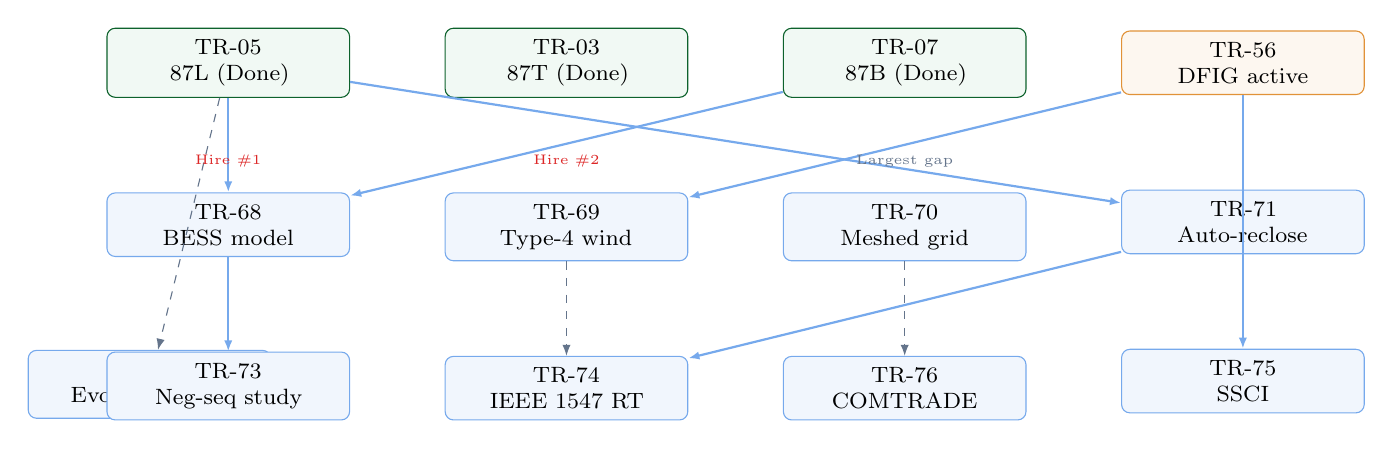
\begin{tikzpicture}[
  node distance=6mm and 12mm,
  box/.style={rectangle, rounded corners=3pt, draw=blue!60, fill=blue!6,
              text width=28mm, align=center, font=\footnotesize, inner sep=4pt},
  done/.style={box, draw=green!60!black, fill=green!6},
  active/.style={box, draw=amber!80, fill=amber!6},
  arr/.style={-{Latex[length=4pt]}, thick, blue!60},
  darr/.style={-{Latex[length=4pt]}, dashed, slate},
]

%% Row 0 — existing
\node[done] (87L)  {TR-05\\87L (Done)};
\node[done, right=of 87L] (87T)  {TR-03\\87T (Done)};
\node[done, right=of 87T] (87B)  {TR-07\\87B (Done)};
\node[active, right=of 87B] (dfig) {TR-56\\DFIG active};

%% Row 1 — Tier 1
\node[box, below=12mm of 87L] (bess)  {TR-68\\BESS model};
\node[box, below=12mm of 87T] (t4)    {TR-69\\Type-4 wind};
\node[box, below=12mm of 87B] (mesh)  {TR-70\\Meshed grid};
\node[box, below=12mm of dfig] (ar)   {TR-71\\Auto-reclose};
\node[box, below=32mm of 87L, xshift=-10mm] (evol) {TR-72\\Evolving faults};

%% Row 2 — Tier 2
\node[box, below=12mm of bess] (negs) {TR-73\\Neg-seq study};
\node[box, below=12mm of t4]   (1547) {TR-74\\IEEE 1547 RT};
\node[box, below=12mm of ar]   (ssci) {TR-75\\SSCI};
\node[box, below=12mm of mesh] (comtr){TR-76\\COMTRADE};

%% Tier 1 arrows
\draw[arr] (87L) -- (bess);
\draw[arr] (87B) -- (bess);
\draw[arr] (dfig) -- (t4);
\draw[arr] (87L) -- (ar);
\draw[darr] (87L) -- (evol);
\draw[darr] (mesh) -- (comtr);

%% Tier 2 arrows
\draw[arr] (bess) -- (negs);
\draw[arr] (ar)   -- (1547);
\draw[arr] (dfig) -- (ssci);
\draw[darr] (t4) -- (1547);

%% Mesh dependency
\node[above=2mm of mesh, font=\tiny\color{slate}] {Largest gap};
\node[above=2mm of bess, font=\tiny\color{red}] {Hire \#1};
\node[above=2mm of t4,   font=\tiny\color{red}] {Hire \#2};

\end{tikzpicture}
\end{center}

%% ════════════════════════════════════════════════════════════
\section{Hiring Profiles}
\label{sec:hiring}

\subsection{Hire \#1 — BESS / Power Electronics Protection (TR-68, TR-74, TR-85)}

\begin{infobox}
\textbf{Title:} Research Engineer / Postdoc — BESS \& IBR Protection \\[4pt]
\textbf{Duration:} 18--24 months \\[4pt]
\textbf{Deliverables:} TR-68 (BESS source model + 87L/87B extension),
TR-74 (IEEE 1547 ride-through compliance study),
TR-85 (cold load pickup).
Journal target: \textit{IEEE Transactions on Power Delivery}. \\[4pt]
\textbf{Required background:}
\begin{itemize}
  \item Grid-scale BESS control (VSM / droop / virtual impedance modes)
  \item Python (NumPy/SciPy); familiarity with PandaPower or ANDES
  \item Protection fundamentals (IEC 60255, percentage-differential relays)
\end{itemize}
\textbf{Nice to have:} Real-time simulator experience (OPAL-RT, RTDS).
\end{infobox}

\subsection{Hire \#2 — Wind (Type-4) \& Subsynchronous Interactions (TR-69, TR-75)}

\begin{infobox}
\textbf{Title:} Research Engineer — Wind IBR Protection \\[4pt]
\textbf{Duration:} 12--18 months \\[4pt]
\textbf{Deliverables:} TR-69 (PMSG Type-4 source model + protection study),
TR-75 (SSCI detection and relay discrimination).
Journal target: \textit{IEEE Transactions on Energy Conversion}. \\[4pt]
\textbf{Required background:}
\begin{itemize}
  \item PMSG / Type-4 converter controls; crowbar-less FRT
  \item ANDES or PSCAD; understanding of subsynchronous resonance
  \item Relay sequence-component analysis (Fortescue)
\end{itemize}
\end{infobox}

\subsection{Hire \#3 — Network Topology \& Wide-Area Protection (TR-70, TR-83)}

\begin{infobox}
\textbf{Title:} Research Engineer — Meshed Network \& Synchrophasor Protection \\[4pt]
\textbf{Duration:} 24 months (largest scope) \\[4pt]
\textbf{Deliverables:} TR-70 (meshed topology, directional 67 relay, pilot scheme),
TR-83 (PMU / C37.118 wide-area backup).
Journal target: \textit{IEEE Transactions on Smart Grid}. \\[4pt]
\textbf{Required background:}
\begin{itemize}
  \item Power system network analysis (meshed load flow, fault analysis in loops)
  \item Directional overcurrent and distance relay coordination
  \item Synchrophasor (PMU) measurement chains; preferably C37.118
\end{itemize}
\end{infobox}

\subsection{Hire \#4 — Cybersecurity \& Communications (TR-82, TR-76)}

\begin{infobox}
\textbf{Title:} Research Engineer — Cyber-Physical Security \\[4pt]
\textbf{Duration:} 12--18 months \\[4pt]
\textbf{Deliverables:} TR-82 (GOOSE attack modelling, IEC 62351 compliance),
TR-76 (COMTRADE data pipeline, field-data validation MOU).
Journal target: \textit{IEEE Transactions on Industrial Informatics}. \\[4pt]
\textbf{Required background:}
\begin{itemize}
  \item IEC 61850 GOOSE / MMS protocol internals
  \item Cyber-physical attack modelling (replay, spoofing, latency injection)
  \item Familiarity with IEC 62351 security for protection
\end{itemize}
\end{infobox}

%% ════════════════════════════════════════════════════════════
\section{Consortium Workpackage Mapping}
\label{sec:consortium}

The table below maps gaps to Horizon Europe / CIGRE workpackage structures.
It is intended as a starting point for a consortium proposal — each WP
corresponds to one or more hires and a coherent set of TRs.

\vspace{4mm}
\begin{center}
\small
\setlength{\tabcolsep}{5pt}
\renewcommand{\arraystretch}{1.4}
\begin{tabular}{@{}L{2.5cm} L{3.5cm} L{3.5cm} C{1.2cm} C{1.2cm}@{}}
\toprule
\textbf{WP} & \textbf{Title} & \textbf{TRs} & \textbf{Effort} & \textbf{Partner fit} \\
\midrule
WP1 & BESS \& GFM Protection & TR-68, 74, 85 & 6 EM & Industry (BESS OEM) \\
WP2 & Type-4 Wind \& SSCI & TR-69, 75 & 6 EM & Wind OEM / TSO \\
WP3 & Meshed Grid \& Directional & TR-70, 83 & 10 EM & TSO / DSO \\
WP4 & Standards Compliance & TR-71, 72, 73, 77, 78, 79 & 10 EM & Relay vendor \\
WP5 & Field Validation & TR-76 & 2 EM & Utility (data MOU) \\
WP6 & Cyber-Physical Security & TR-82 & 3 EM & Cybersecurity partner \\
WP7 & Emerging Topics & TR-80, 81, 84 & 10 EM & Academic partners \\
\midrule
\multicolumn{3}{@{}l}{\textbf{Total}} & \textbf{47 EM} & \\
\bottomrule
\end{tabular}
\end{center}

\begin{warnbox}
\textbf{Critical path to Q3 2028 submission.}
TR-68 (BESS) is the single most important new TR before submission. It closes the
largest source-type gap and produces a chapter-length study. Hire~\#1 must be
onboarded by \textbf{Q4 2026} to leave sufficient time for TR-68 + journal submission
before the thesis lock date.

TR-70 (meshed grid) is the largest structural gap but is \emph{not} on the critical
path — it is scoped as post-thesis consortium work and explicitly bounded in
Chapter~10.
\end{warnbox}

%% ════════════════════════════════════════════════════════════
\section{What Is Not a Gap (Scope Bounds)}

The following items were considered and deliberately excluded:

\begin{itemize}
  \item \textbf{HVDC protection:} Out of scope for a microgrid/distribution
        protection thesis; a separate HVDC protection programme is warranted.
  \item \textbf{Arc-flash detection:} Overlap with occupational safety standards
        (NFPA 70E / IEC 62271); not a relay protection problem in the SAMBP sense.
  \item \textbf{Stator ground fault (64S) for synchronous machines:} Covered
        adequately by existing 64G work; marginal additional value.
  \item \textbf{Load shedding (UFLS) schemes:} System-stability function, not a
        selective protection function; separate discipline.
  \item \textbf{PSCAD as primary simulator:} ANDES + PandaPower + OpenDSS cover the
        required fidelity range. PSCAD is used in Ch.~6 data generation only;
        no additional PSCAD integration is planned.
\end{itemize}

%% ════════════════════════════════════════════════════════════
\section{Document Maintenance}

This document should be updated:
\begin{itemize}
  \item When a TR changes status (Planned $\to$ Active $\to$ Done).
  \item When a new hire is confirmed — assign TRs and update effort column.
  \item When a consortium proposal is submitted — attach WP mapping as appendix.
  \item Quarterly review cadence recommended; owner: Anoop V Eluvathingal.
\end{itemize}

\vspace{6mm}
\noindent\textcolor{slate}{\rule{\linewidth}{0.3pt}}\\[3pt]
{\small\textcolor{slate}{%
  Smart Grid Computational Research Lab (SGCRL), IIT Madras $\cdot$ Prof.\ K.\ Shanti Swarup $\cdot$
  Internal Draft v1.0 $\cdot$ April 2026 $\cdot$
  Not for external distribution without review.%
}}

\end{document}
